% PCT-SOURCE: pdf=210 print=198 kind=figure id=A.3
% Native reconstruction of the state profiles and automorphism arrows on
% source page 198.  The curves are schematic profiles, as in the source.
\begingroup
\renewcommand{\thefigure}{A.3}
\renewcommand{\figurename}{Figure}
\begin{figure}[p]
  \centering
\resizebox{\textwidth}{!}{%
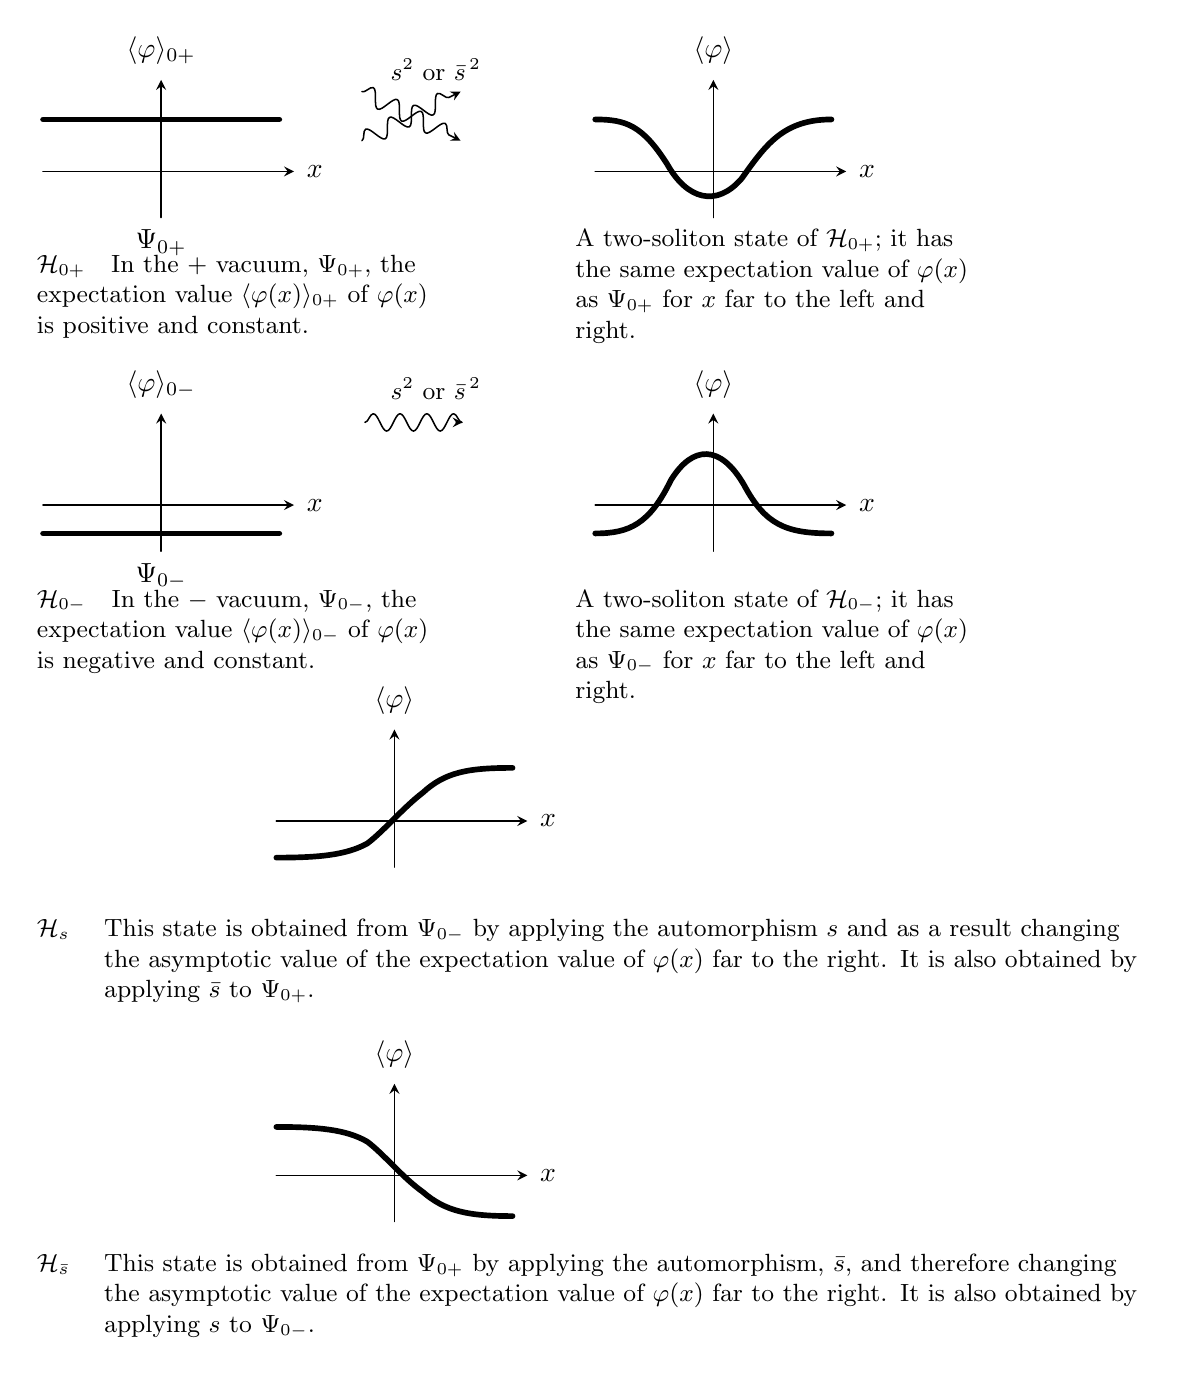
\begin{tikzpicture}[x=.75cm,y=.75cm,>=stealth,line cap=round,
    line join=round]
    % Reusable axes for the four small profiles.
    \newcommand{\pctaxes}[1]{%
      \draw[->,line width=.6pt] (#1-2.0,0) -- (#1+2.25,0)
        node[right=1pt] {$x$};%
      \draw[->,line width=.6pt] (#1, -.78) -- (#1,1.55);%
    }

    % Top-left: the positive vacuum.
    \begin{scope}[shift={(2.35,13.2)}]
      \pctaxes{0}
      \draw[line width=2.05pt] (-2.0,.88) -- (2.0,.88);
      \node[above=2pt] at (0,1.55) {$\langle\varphi\rangle_{0+}$};
      \node[below=1pt] at (0,-.78) {$\Psi_{0+}$};
    \end{scope}
    \node[anchor=north west,text width=5.2cm,align=left,font=\small]
      at (.08,11.95) {$\mathcal H_{0+}$\quad In the $+$ vacuum, $\Psi_{0+}$, the expectation value $\langle\varphi(x)\rangle_{0+}$ of $\varphi(x)$ is positive and constant.};

    % Top-right: a two-soliton profile in the positive sector.
    \begin{scope}[shift={(11.7,13.2)}]
      \pctaxes{0}
      \draw[line width=2.05pt]
        (-2.0,.88) .. controls (-1.48,.88) and (-1.20,.78) .. (-.78,.12)
        .. controls (-.45,-.47) and (.05,-.62) .. (.48,-.12)
        .. controls (.88,.44) and (1.18,.88) .. (2.0,.88);
      \node[above=2pt] at (0,1.55) {$\langle\varphi\rangle$};
    \end{scope}
    \node[anchor=north west,text width=5.15cm,align=left,font=\small]
      at (9.2,12.38) {A two-soliton state of $\mathcal H_{0+}$; it has the same expectation value of $\varphi(x)$ as $\Psi_{0+}$ for $x$ far to the left and right.};

    % The crossed wavy arrows between the first row of panels.
    \node[font=\small] at (7.0,14.92) {$s^2$ or $\bar s^{\,2}$};
    \draw[->,line width=.55pt,decorate,
      decoration={snake,amplitude=.11cm,segment length=.34cm}]
      (5.75,14.55) -- (7.42,13.72);
    \draw[->,line width=.55pt,decorate,
      decoration={snake,amplitude=.11cm,segment length=.34cm}]
      (5.75,13.72) -- (7.42,14.55);

    % Middle-left: the negative vacuum.
    \begin{scope}[shift={(2.35,7.55)}]
      \pctaxes{0}
      \draw[line width=2.05pt] (-2.0,-.48) -- (2.0,-.48);
      \node[above=2pt] at (0,1.55) {$\langle\varphi\rangle_{0-}$};
      \node[below=1pt] at (0,-.78) {$\Psi_{0-}$};
    \end{scope}
    \node[anchor=north west,text width=5.2cm,align=left,font=\small]
      at (.08,6.28) {$\mathcal H_{0-}$\quad In the $-$ vacuum, $\Psi_{0-}$, the expectation value $\langle\varphi(x)\rangle_{0-}$ of $\varphi(x)$ is negative and constant.};

    % Middle-right: a two-soliton profile in the negative sector.
    \begin{scope}[shift={(11.7,7.55)}]
      \pctaxes{0}
      \draw[line width=2.05pt]
        (-2.0,-.48) .. controls (-1.42,-.48) and (-1.08,-.32) .. (-.72,.42)
        .. controls (-.35,1.02) and (.12,1.03) .. (.52,.34)
        .. controls (.88,-.33) and (1.22,-.48) .. (2.0,-.48);
      \node[above=2pt] at (0,1.55) {$\langle\varphi\rangle$};
    \end{scope}
    \node[anchor=north west,text width=5.15cm,align=left,font=\small]
      at (9.2,6.28) {A two-soliton state of $\mathcal H_{0-}$; it has the same expectation value of $\varphi(x)$ as $\Psi_{0-}$ for $x$ far to the left and right.};

    % The single wavy arrow in the second row.
    \node[font=\small] at (7.0,9.52) {$s^2$ or $\bar s^{\,2}$};
    \draw[->,line width=.55pt,decorate,
      decoration={snake,amplitude=.11cm,segment length=.34cm}]
      (5.8,8.95) -- (7.45,8.95);

    % Profile obtained by applying s to the positive vacuum.
    \begin{scope}[shift={(6.3,2.2)}]
      \pctaxes{0}
      \draw[line width=2.05pt]
        (-2.0,-.62) .. controls (-1.3,-.62) and (-.82,-.58) .. (-.46,-.38)
        .. controls (-.18,-.17) and (.14,.22) .. (.48,.48)
        .. controls (.86,.83) and (1.25,.9) .. (2.0,.9);
      \node[above=2pt] at (0,1.55) {$\langle\varphi\rangle$};
    \end{scope}
    \node[anchor=north west,text width=1.0cm,align=left,font=\small]
      at (.08,.7) {$\mathcal H_s$};
    \node[anchor=north west,text width=13.2cm,align=left,font=\small]
      at (1.22,.7) {This state is obtained from $\Psi_{0-}$ by applying the automorphism $s$ and as a result changing the asymptotic value of the expectation value of $\varphi(x)$ far to the right. It is also obtained by applying $\bar s$ to $\Psi_{0+}$.};

    % Profile obtained by applying s to the negative vacuum.
    \begin{scope}[shift={(6.3,-3.8)}]
      \pctaxes{0}
      \draw[line width=2.05pt]
        (-2.0,.82) .. controls (-1.3,.82) and (-.82,.78) .. (-.46,.57)
        .. controls (-.18,.36) and (.14,-.04) .. (.48,-.28)
        .. controls (.86,-.61) and (1.25,-.69) .. (2.0,-.69);
      \node[above=2pt] at (0,1.55) {$\langle\varphi\rangle$};
    \end{scope}
    \node[anchor=north west,text width=1.0cm,align=left,font=\small]
      at (.08,-4.97) {$\mathcal H_{\bar s}$};
    \node[anchor=north west,text width=13.2cm,align=left,font=\small]
      at (1.22,-4.97) {This state is obtained from $\Psi_{0+}$ by applying the automorphism, $\bar s$, and therefore changing the asymptotic value of the expectation value of $\varphi(x)$ far to the right. It is also obtained by applying $s$ to $\Psi_{0-}$.};
  \end{tikzpicture}%
}
  \caption{\sloppy Behavior of $\langle\varphi(x)\rangle$ as a function of space coordinate for some typical states of $\mathcal{P}(\varphi^4)_2$ in the two-phase region. The action of the automorphisms $s^2=s\circ s$, $\bar{s}^{\,2}=\bar{s}\circ\bar{s}$ and $s\circ\bar{s}$ are indicated by the wavy arrows. In particular, note that the action of the composite automorphism $s\circ\bar{s}$ is to change the asymptotic value of the expectation value of $\varphi(x)$ both to the right and left.}
  \label{fig:A-3}
\end{figure}
\endgroup
